\documentclass{beamer}

\usepackage[font=footnotesize]{subcaption}
\usepackage{graphicx}
\usepackage{siunitx}
\usepackage[utf8]{inputenc}
\usepackage{mathtools}
\usepackage{enumerate}
\setbeamertemplate{frametitle}[default][left]
\usetheme[width=2.1cm]{Hannover}
\usefonttheme{serif}     % Font theme: serif
\usepackage{ccfonts}     % Font family: Concrete Math
\usepackage[T2]{fontenc} % Font encoding: T1
%Information to be included in the title page:
\title{Differential Capacitance of Ionic Liquid Interface with Graphene: The Effects of Correlation and Finite Size of
Ions}
\author{Ahmed Shalabi}
\institute{University of Waterloo \\ 
Department of Physics and Astronomy}
\date{August 19, 2019}
 
 
 
\begin{document}
\allowdisplaybreaks
%%%%%%%%%%%%%%%%%%%%% Title page %%%%%%%%%
\begin{frame}
\titlepage
\end{frame}

%%%%%%%%%%%%%%%%%%%%%% Intro %%%%%%%%%%%%%%%%%%%%%%%%%%%%%%
\section{Introduction}
\begin{frame}{Outline}

\begin{itemize}
\item \textcolor{red}{Background and Motivation}\\
\item Ionic Liquids\\
\item Graphene Electrodes\\
\item Computational approach \\
\item Results \\
\item Conclusions and Future Work
\end{itemize}
\end{frame}
%%%%%%%%%%%%%%%%%%%%%%%% Background and Motivation %%%%%%%%%%
\section{Background and Motivation}
\begin{frame}{Background and Motivation}
Graphene:
\begin{itemize}
    \item High mobility of charge carriers in $\pi$ electron bonds
    \item Zero-Energy band gap
    \item Dirac cone approximation
    \item Operate as field effective transistors
\end{itemize}
   \begin{figure}[!ht]
     \begin{subfigure}[b]{0.45\linewidth}
       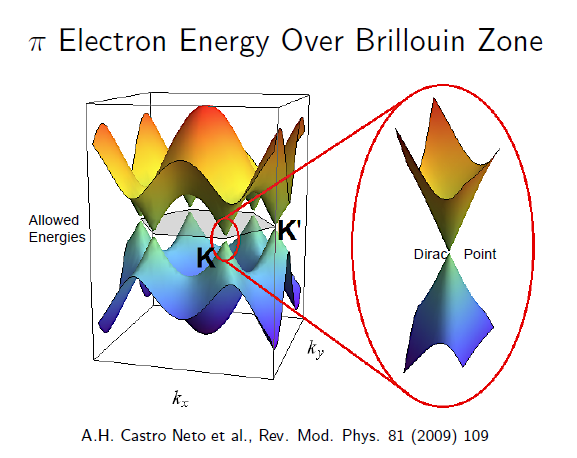
\includegraphics[width=\linewidth]{band_struct.PNG}
     \end{subfigure}
     \hfill
     \begin{subfigure}[b]{0.45\linewidth}
       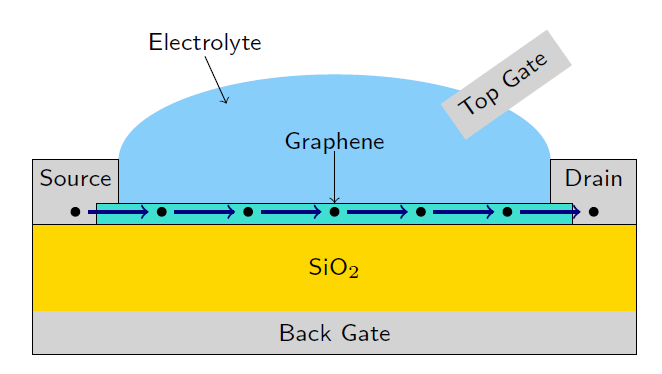
\includegraphics[width=\linewidth]{FET.PNG}
     \end{subfigure}
   \end{figure}
\end{frame}
%%%%%%%%%%%%%%%%%%%%%%% Ionic liquids %%%%%%%%%%%%%%%%%%
\begin{frame}{Outline}

\begin{itemize}
\item Background and Motivation\\
\item \textcolor{red}{Ionic Liquids}\\
\item Graphene Electrodes\\
\item Computational approach \\
\item Results \\
\item Conclusions and Future Work
\end{itemize}
\end{frame}

\section{Ionic Liquids}
\begin{frame}{Ionic Liquids}
    \begin{center}
        \begin{figure}
            \centering
            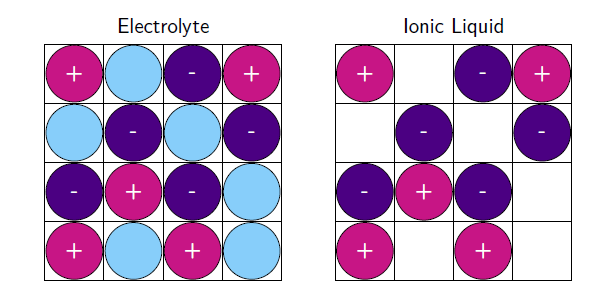
\includegraphics[scale=0.5]{ILs.PNG}
        \end{figure}{}
    \end{center}{}

    \begin{itemize}
        \item Melting points below 100 C
        \item Comprised strictly of positive and negative ions
        \item High conductivity and lower volatility than typical electrolytes
        \item Inter ionic correlations and overscreening 
    \end{itemize}{}
\end{frame}

\subsection{Free Energy and The Modifided Poisson Fermi equation}

\begin{frame}{Free energy functional}
Gibbs Free Energy:
$$F = U - TS$$
Functional for ionic liquids:
$$ F = \int \bigg[ -\frac{\varepsilon}{8\pi}(|\nabla \phi |^2 +l_c^2(\nabla^2 \phi)^2) +\rho \phi -TS \bigg] d^3r $$
where the charge density $\rho$ is defined as:
$$\rho = e(z_+c_+ - z_-c_-)$$
with the entropic term:
\begin{multline*}
-TS = \frac{K_BT}{v}[vc_- \ln{(vc_- )} + vc_+ \ln{(vc_+)} \\+ (1 -vc_- - vc_+)\ln{(1 - vc_- -vc_+)}]
\end{multline*}
\end{frame}

\begin{frame}{Poisson Fermi equation}
Minimization w.r.t the concentration yields:
$$c_{\pm} = \frac{c_{\infty}e^{\pmze\beta\phi}}{1 - \gamma + \gamma \cosh{(ze\beta\phi)}} $$
where $c_{\infty}$ is the concentration in the neutral bulk, $\beta = \frac{1}{K_BT}$ and $\gamma = 2vc_{\infty}$ defines the ionic packing fraction\\
\vspace{1em}
Minimization w.r.t the potential yields:
$$(1 - \delta_c^2 \nabla^2)\nabla^2 \phi = -4\pi\rho$$
with $\delta_c = \frac{l_c}{\lambda_D}$ is a dimensionless correlation length with $\lambda_D$ defining the Debye length in the ionic liquid
\end{frame}

\subsection{Differential Capacitance}
\begin{frame}{Differential Capacitance in the Diffuse Layer}
Charge density per unit area:
    $$\sigma_d(\phi_0) = \int^\infty_0 \rho(\phi(x);\phi_0)dx $$
    Apply external voltage to the bulk resulting in a potential drop across the diffuse layer:
    $$V_d = -\phi_0$$
    Differential capacitance per unit area:
    $$C_d = \frac{d\sigma_d}{dV_d}$$
\end{frame}{}

\subsection{1D Problem}
\begin{frame}{1D Problem}
\begin{itemize}
    \item Exploit the planar geometry to solve a 1D the modified Poisson Boltzmann equation:
$$ \phi^{''} - \delta_c^2 \phi^{''''} = -4\pi \rho(\phi)$$
which the BCs:
$$ \phi(0) = \phi_0 , \phi(0)^{'''} = 0 , \phi^{'}(\infty) = 0, \phi^{'''}(\infty) = 0 $$
\item Inclusion of Graphene requires non trivial changes to the Boundary conditions.
\item Utilize the charge neutrality condition.
\end{itemize}{}
\end{frame}

%%%%%%%%%%%%%%%%%%%%%%%%%%%

\begin{frame}{Outline}

\begin{itemize}
\item Background and Motivation\\
\item Ionic Liquids\\
\item \textcolor{red}{Graphene Electrodes}\\
\item Computational approach \\
\item Results \\
\item Conclusions and Future Work
\end{itemize}
\end{frame}


\section{Graphene}
\subsection{Quantum capacitance}
\begin{frame}
\frametitle{Graphene electrode}
Density of States:\\
$$D(\varepsilon) = \iint \frac{g}{(2 \pi)^2} \delta(\varepsilon - \varepsilon (\vec{k}))d^2\vec{k} $$
which can be linearized by the Dirac Cone approximation to give:\\
$$D(\varepsilon) \approx \frac{2 |\varepsilon|}{\pi (\hbar v_F)^2}$$\\
Charge Density on Graphene: \\
$$\sigma_g(\varepsilon_F) = -e \int D(\varepsilon) \bigg[ \frac{1}{1+e^{\beta(\varepsilon-\varepsilon_F)}} - \frac{1}{1+e^{\beta \varepsilon}} \bigg] d\varepsilon$$
\end{frame}
 

\begin{frame}
Then we define the differential capacitance per unit area i.e the quantum capacitance as: $$C_g = -e \frac{d\sigma_g}{d\varepsilon_F} $$ \\
which gives the following expression for $C_g$:
$$C_g = 2 \Gamma_g \ln[2\cosh{\frac{\beta e V_g}{2}}] $$
where $\Gamma_g = \frac{2 \alpha^2}{\pi e^2 \beta}$, with $\alpha = \frac{e^2}{\hbar v_F}$, $v_F \approx 10^6 m/s$ and $V_g=\mu_c/e$\\
\vspace{1em}
\end{frame}

\subsection{Charge Neutrality}
\begin{frame}{The Neutrality Condition}
Applied potential:
$$V_a = V_d + V_g $$ \\
Charge neutrality condition:
$$\sigma_d(V_d) + \sigma_g(V_g) = 0 $$
Therefore, we can impose the charge neutrality condition to find the relationship between $V_d$ and $V_g$ to find
the total capacitance $C_{dg} = \frac{d\sigma_d}{dV_a}$ as:
$$C_{dg} = [C_{d}(V_d)^{-1} + C_g(V_g)^{-1}]^{-1}$$

\end{frame}
\begin{frame}{Inclusion of a Stern Layer}
%%Applied potential now becomes:
%$$V_a = V_d + V_s + V_g $$ \\
%with $V_s$ defined as:
%$$V_s = \frac{\sigma_d(V_d)}{C_s}$$
%which yields the following total capacitance $C_{dsg} = \frac{d\sigma_d}{dV_a}$ in terms of the diffuse, quantum and Stern layer capacitances:
\begin{figure}[!h]
    \begin{center}
    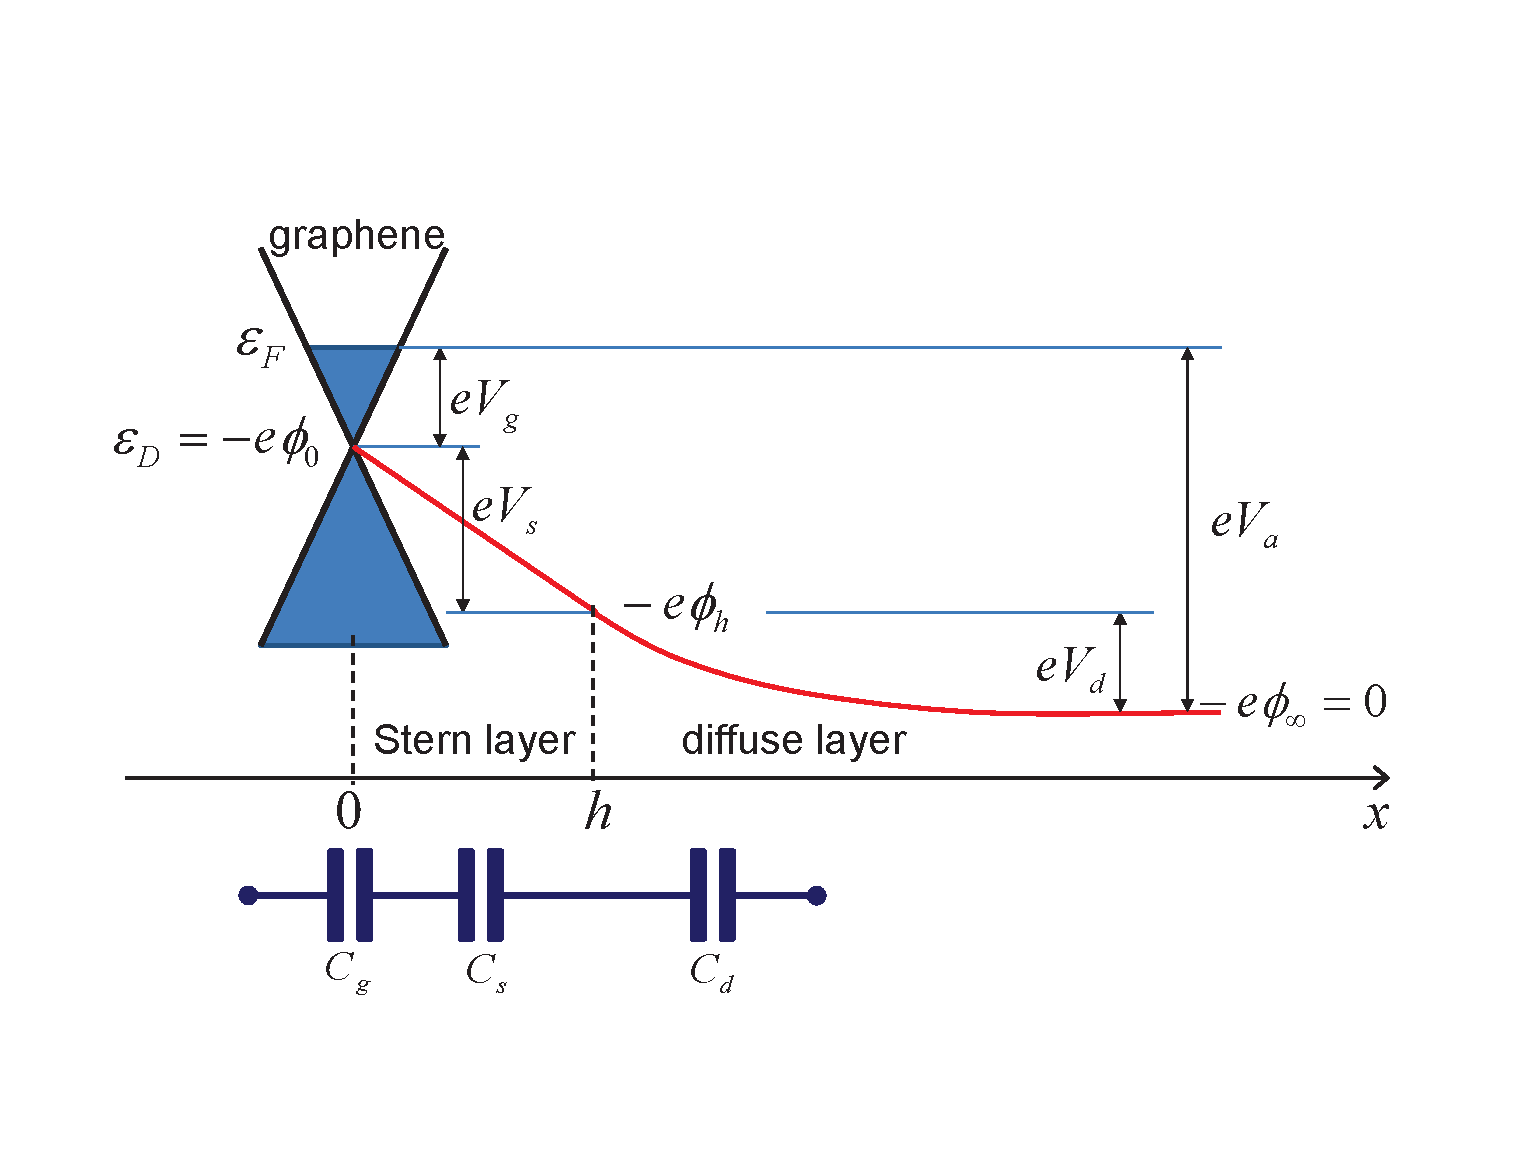
\includegraphics[scale=0.27]{graphenepotential.eps}
    \end{center}
\end{figure}
$$V_s = \frac{\sigma_d}{C_s}$$
$$C_s=\epsilon_s/(4\pi h)$$
$$C_{dsg} = [C_{d}(V_d)^{-1} + C_s ^{-1} + C_g(V_g)^{-1}]^{-1}$$

\end{frame}{}

%%%%%%%%%%%%%%%%%%%%%%%%%%%%%%%%%%%%%%%%%%%%%%%%%%%%%%
\begin{frame}{Outline}

\begin{itemize}
\item Background and Motivation\\
\item Ionic Liquids\\
\item Graphene Electrodes\\
\item \textcolor{red}{Computational approach} \\
\item Results \\
\item Conclusions and Future Work
\end{itemize}
\end{frame}

\section{Computational Approach}
\subsection{Algorithm}
\begin{frame}{Computational approach: Algorithm}
\begin{itemize}
    \item Solve the modified Poisson Fermi equation for an array of initial potential values $\phi_0$ 
    \item For each $\phi_0$ value we find $\rho(\phi(x);\phi_0)$
    \item Numerically integrate to obtain $\sigma_d(\phi_0) = \int \rho dx$
    \item Define $V_d \equiv - \phi_0$ and interpolate the set of $V_d$ and $\sigma_d$ values to obtain a numerical approximation of $\sigma_d(V_d)$
    \item Impose the charge neutrality condition $\sigma_d(V_d) + \sigma_g(V_g) = 0 $ and solve for $V_d(V_a)$ and $V_g(V_a)$, using $V_a = V_d + V_s +V_g$
    \item Calculate $C_d , C_s, C_g$ and $C_{dsg}$ using the expressions derived for the capacitances.
\end{itemize}
\end{frame}

%%%%%%%%%%%%%%%%%%%%%%% Results %%%%%%%%%%%%%%%%%%%%%%%%%%%%%%%%
\begin{frame}{Outline}

\begin{itemize}
\item Background and Motivation\\
\item Ionic Liquids\\
\item Graphene Electrodes\\
\item Computational approach \\
\item \textcolor{red}{Results} \\
\item Conclusions and Future Work
\end{itemize}
\end{frame}

\section{Results}
\begin{frame}{Diffuse Layer Capacitance $C_d$}
    \begin{figure}[!h]
    \begin{center}
    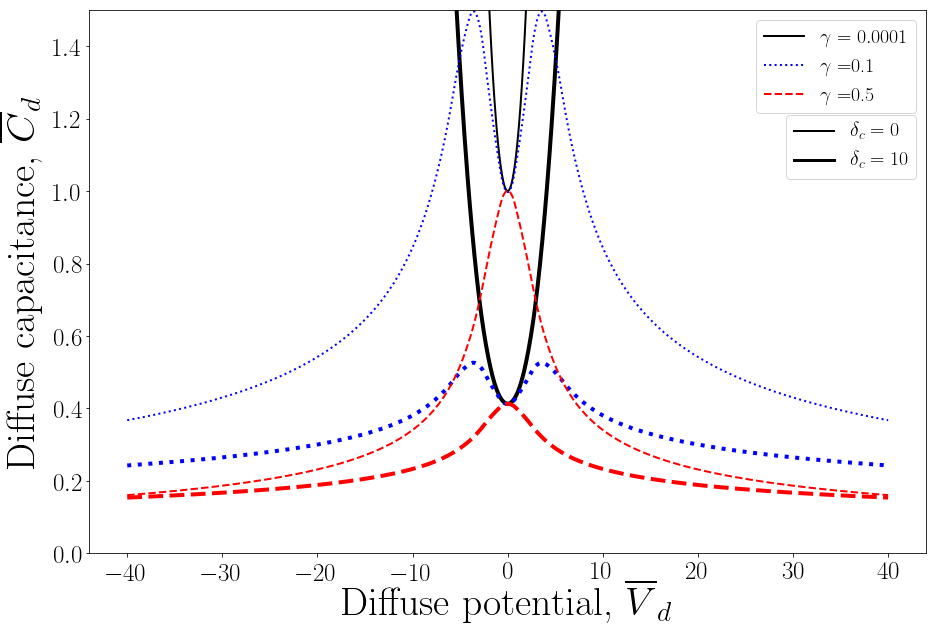
\includegraphics[scale=0.2]{figure_3.png}
    \end{center}
    \end{figure}
    \begin{itemize} 
    \item Bell and camel shaped capacitances
    \item Ion correlations reduce the capacitance
    \item Independence of $\overline{C}_d$ from $\delta_c$ for large $\gamma$ at large $|\overline{V}_d|$
    \end{itemize}
\end{frame}

\begin{frame}{Double Layer capacitance $C_{ds}$}
    \begin{figure}[!h]
    \begin{center}
    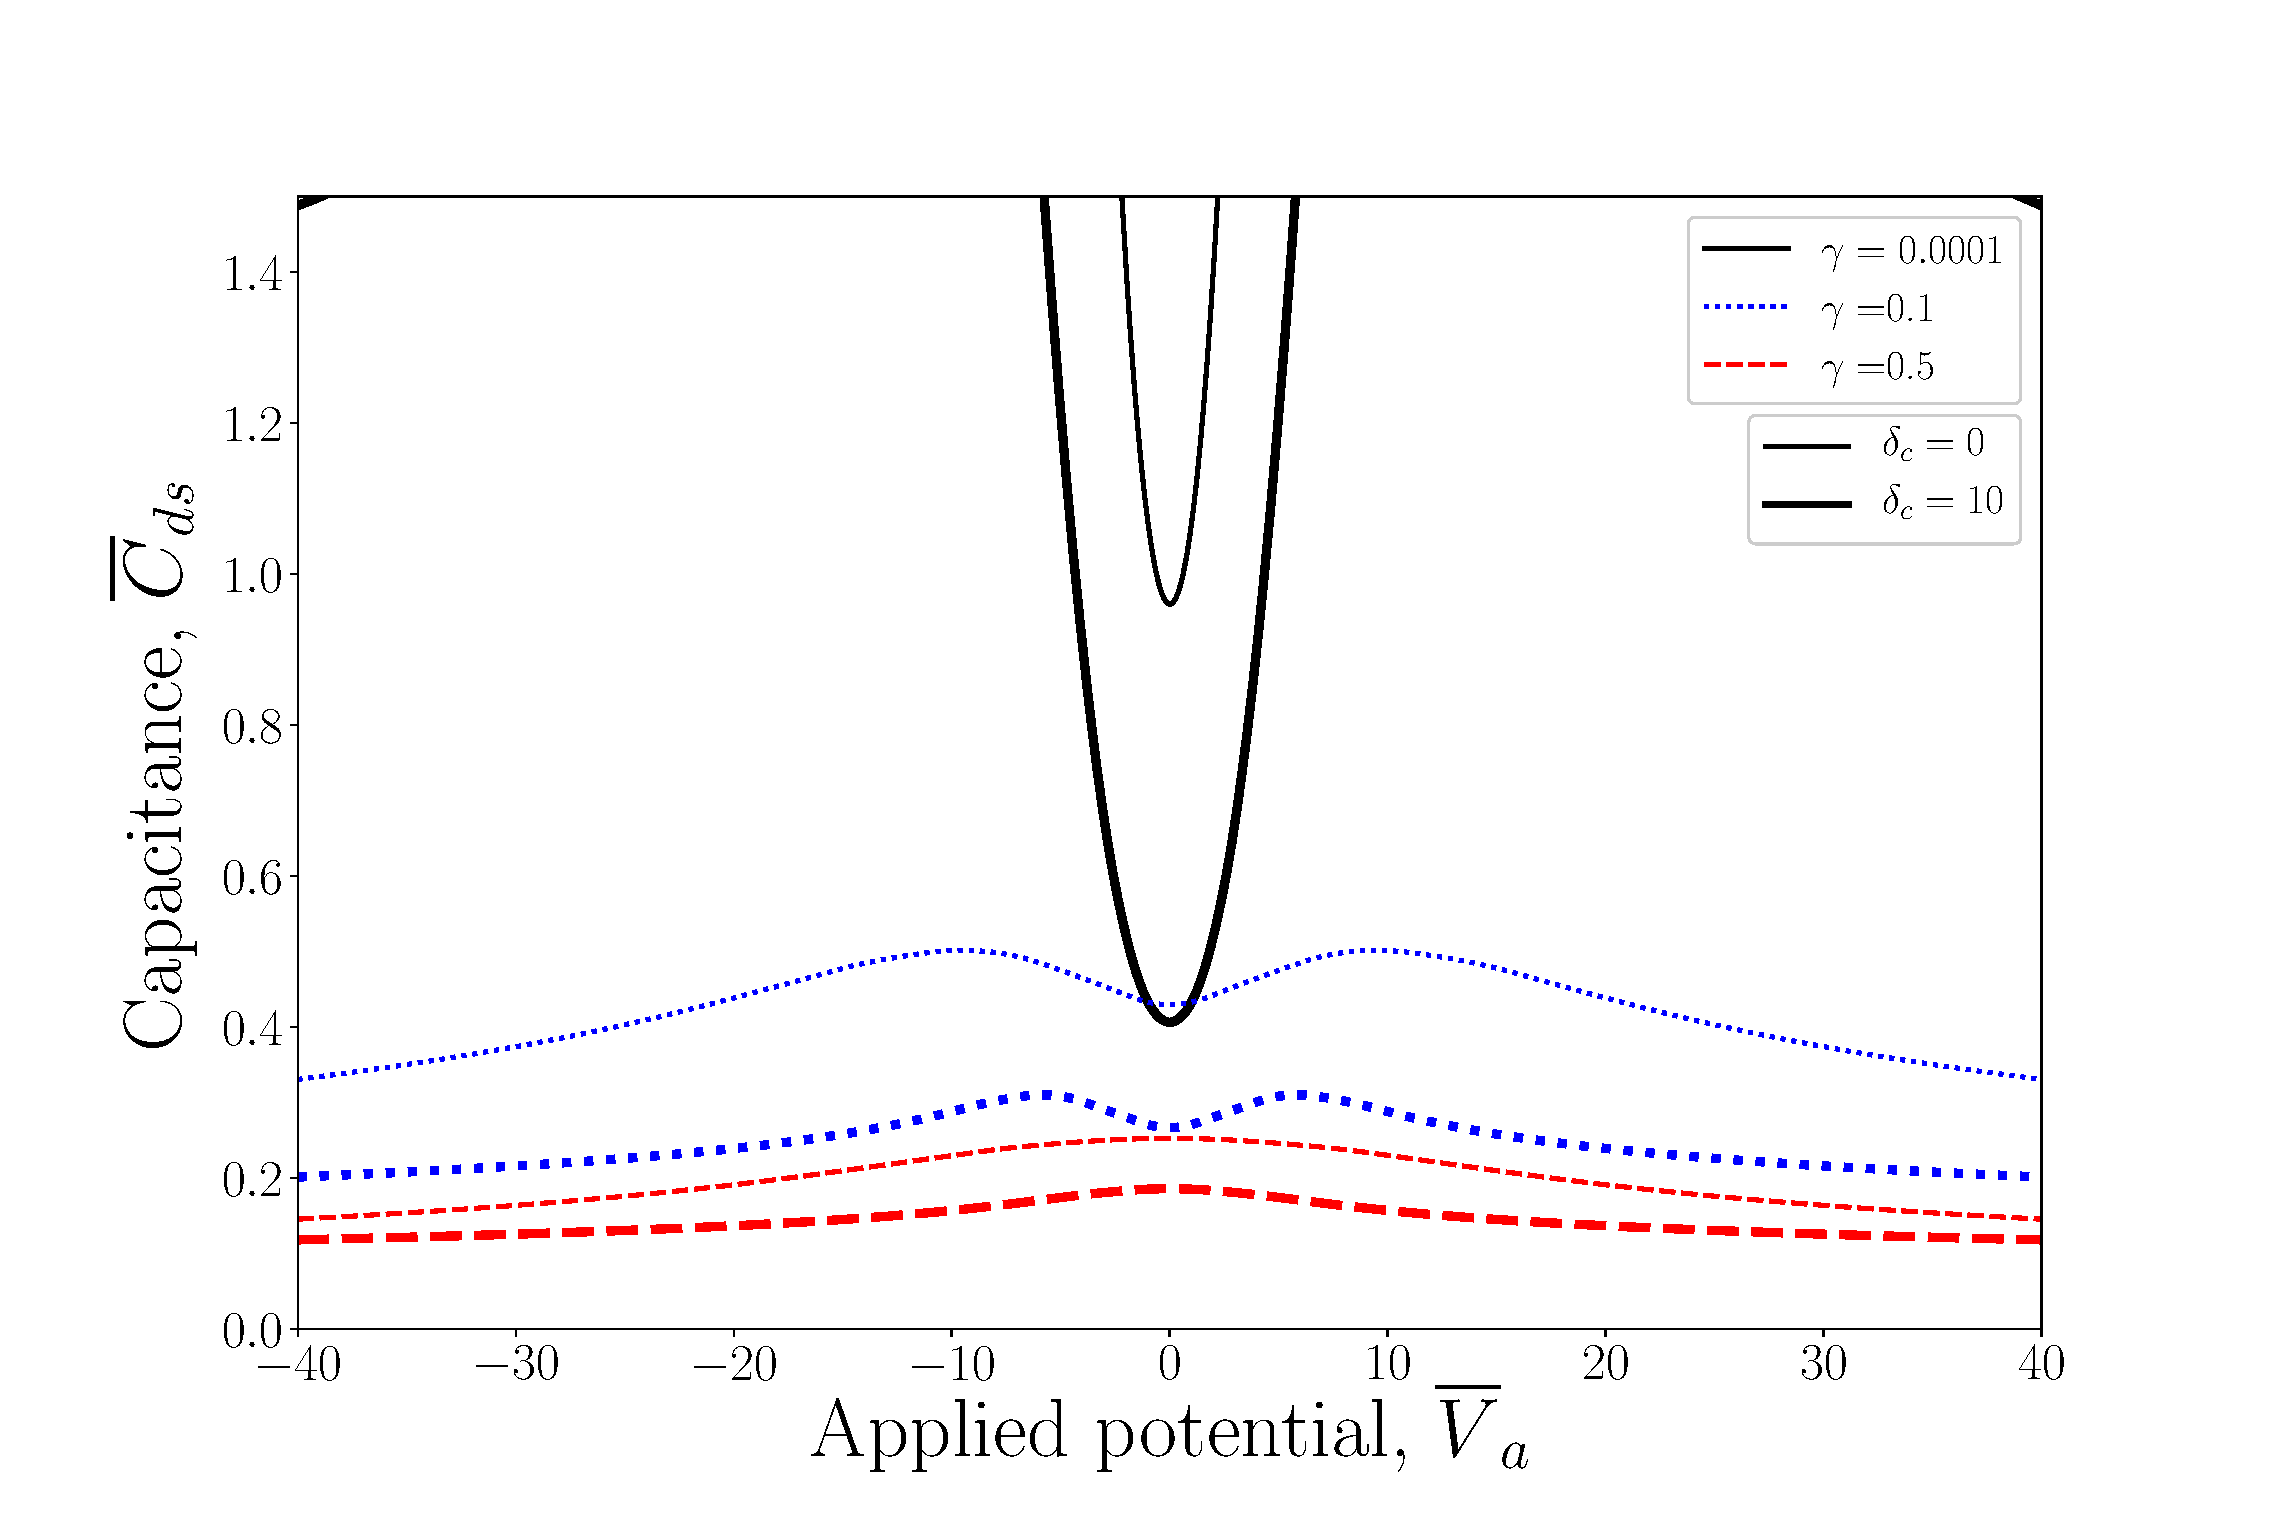
\includegraphics[scale=0.2]{figure_3c.eps}
    \end{center}
    \end{figure}
\begin{itemize}
    \item Inclusion of Stern layer lowers and broadens the capacitance peaks 
\end{itemize}{}
\end{frame}{}

\begin{frame}{Fraction of the total applied potential in diffuse layer, $V_a=V_d+V_g$}
    \begin{figure}[!h]
    \begin{center}
    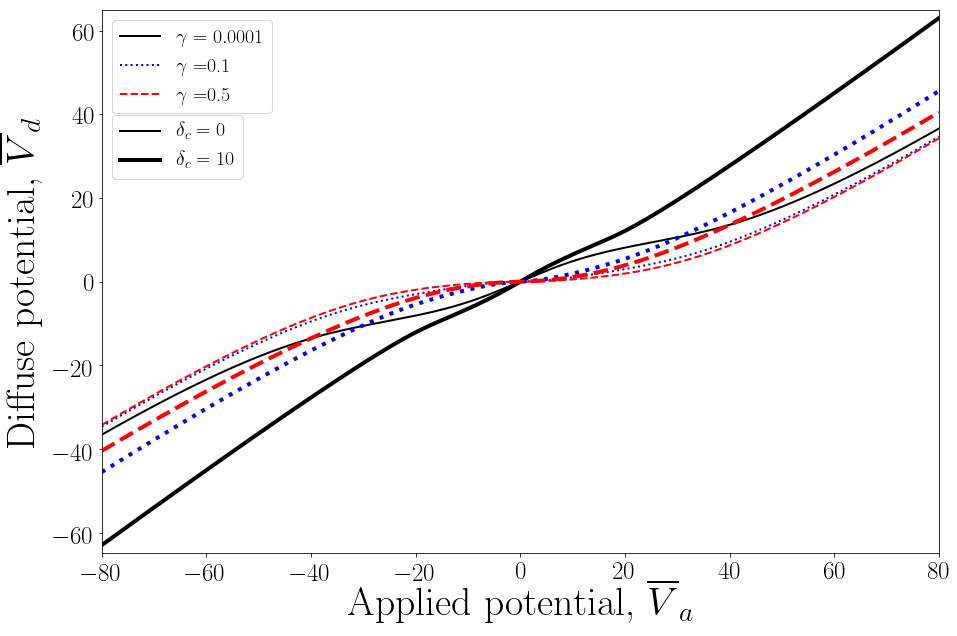
\includegraphics[scale=0.15]{figure_4.png}
    %\caption{ The normalized diffuse potential, $\overline{V}_d$, for a graphene electrode versus the normalized applied potential, $\overline{V}_a $, For no Stern layer on the left vs with one on the right.}
    %\label{Fig4}
    \end{center}
\end{figure}
\begin{itemize}
    \item Most of $\overline{V}_a$ goes to $\overline{V}_g$ i.e charging the graphene electrode
    \item $|\overline{V}_d|$ decreases with increasing $\gamma$ and lowering $\delta_c$
    \item Ion correlations makes the differences for $\overline{V}_d$ for different $\gamma$ more pronounced.
\end{itemize}{}
\end{frame}{}

\begin{frame}{Total Capacitances, $C_{dg}$ and $C_{dsg}$}
   \begin{figure}[!h]
    \begin{center}
    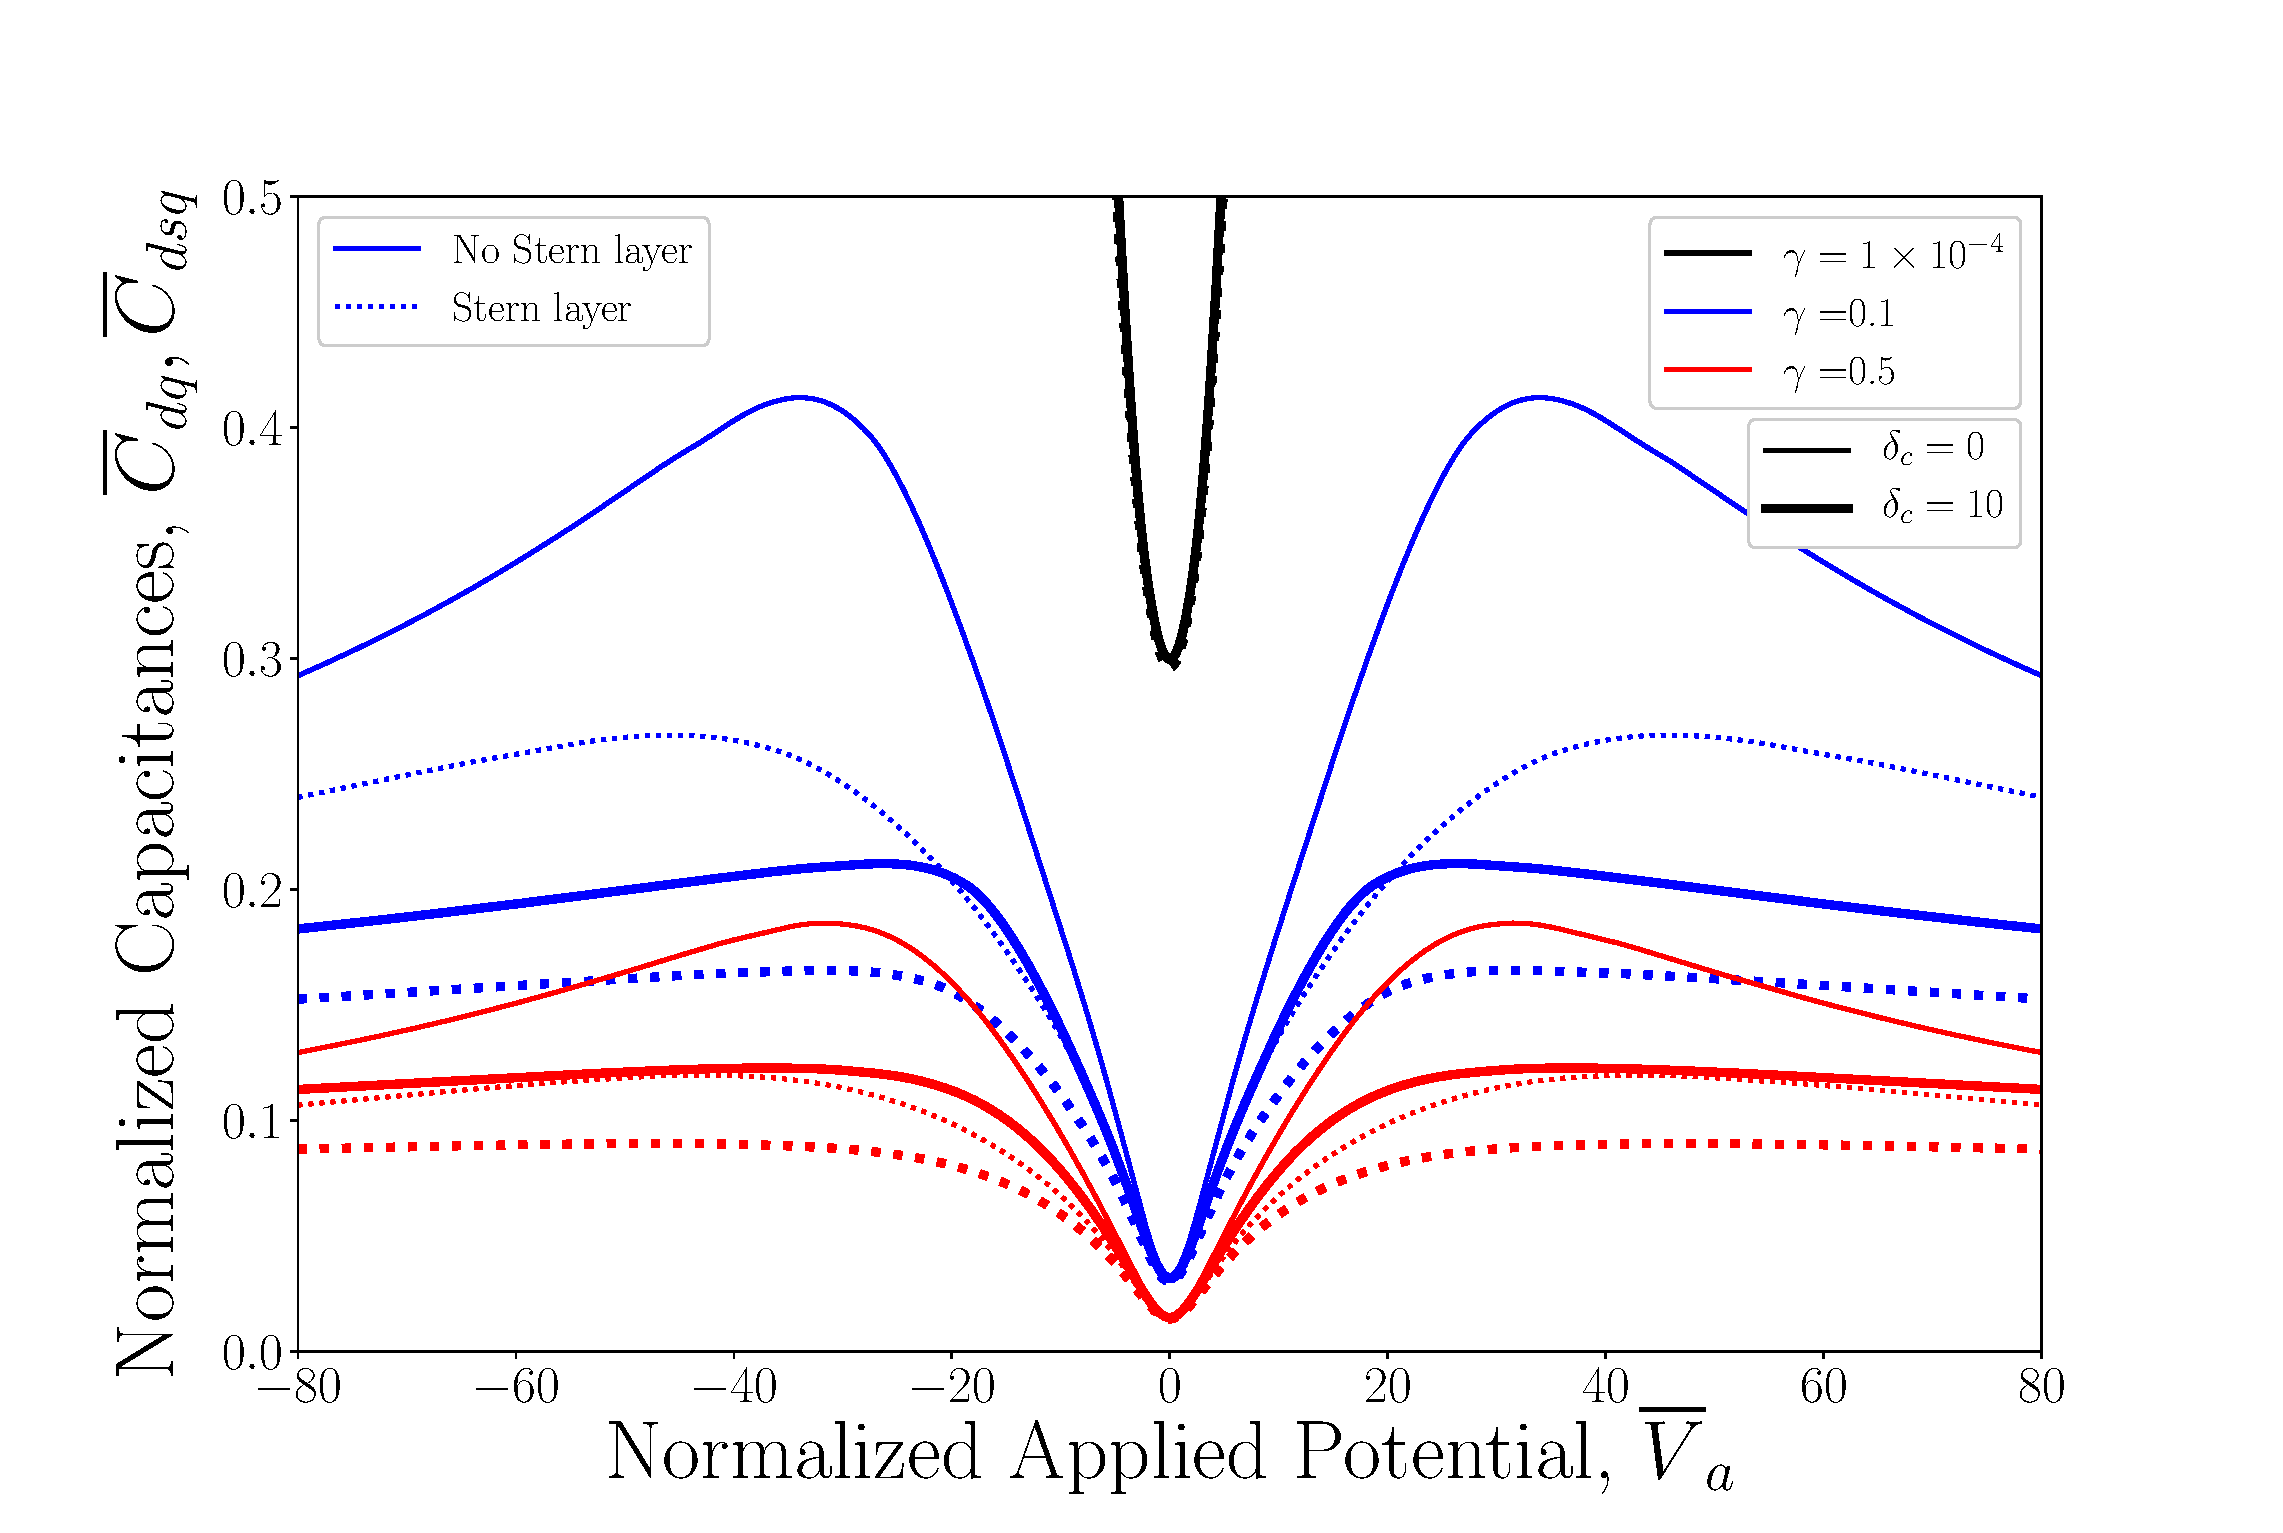
\includegraphics[scale=0.15]{figure_6.eps}
    %\caption{The normalized total capacitances $\overline{C}_{dq}$ and $\overline{C}_{dsq}$ for a graphene electrode with and without a Stern layer. }
    %\label{Fig6}
    \end{center}
\end{figure}
\begin{itemize}
    \item $\overline{C}_g$ dominating the total capacitance around the PZC
    \item Broad peaks and camel shaped dependence for $|\overline{V}_a| >> 10$ for both $\gamma = 0.1$ and $0.5$
    \item Stern layer and ion correlations broaden the overall capacitance
\end{itemize}{} 
\end{frame}{}

\begin{frame}{Asymmetric Ionic Liquid: Charge density}
     \begin{figure}[!h]
        \begin{center}
        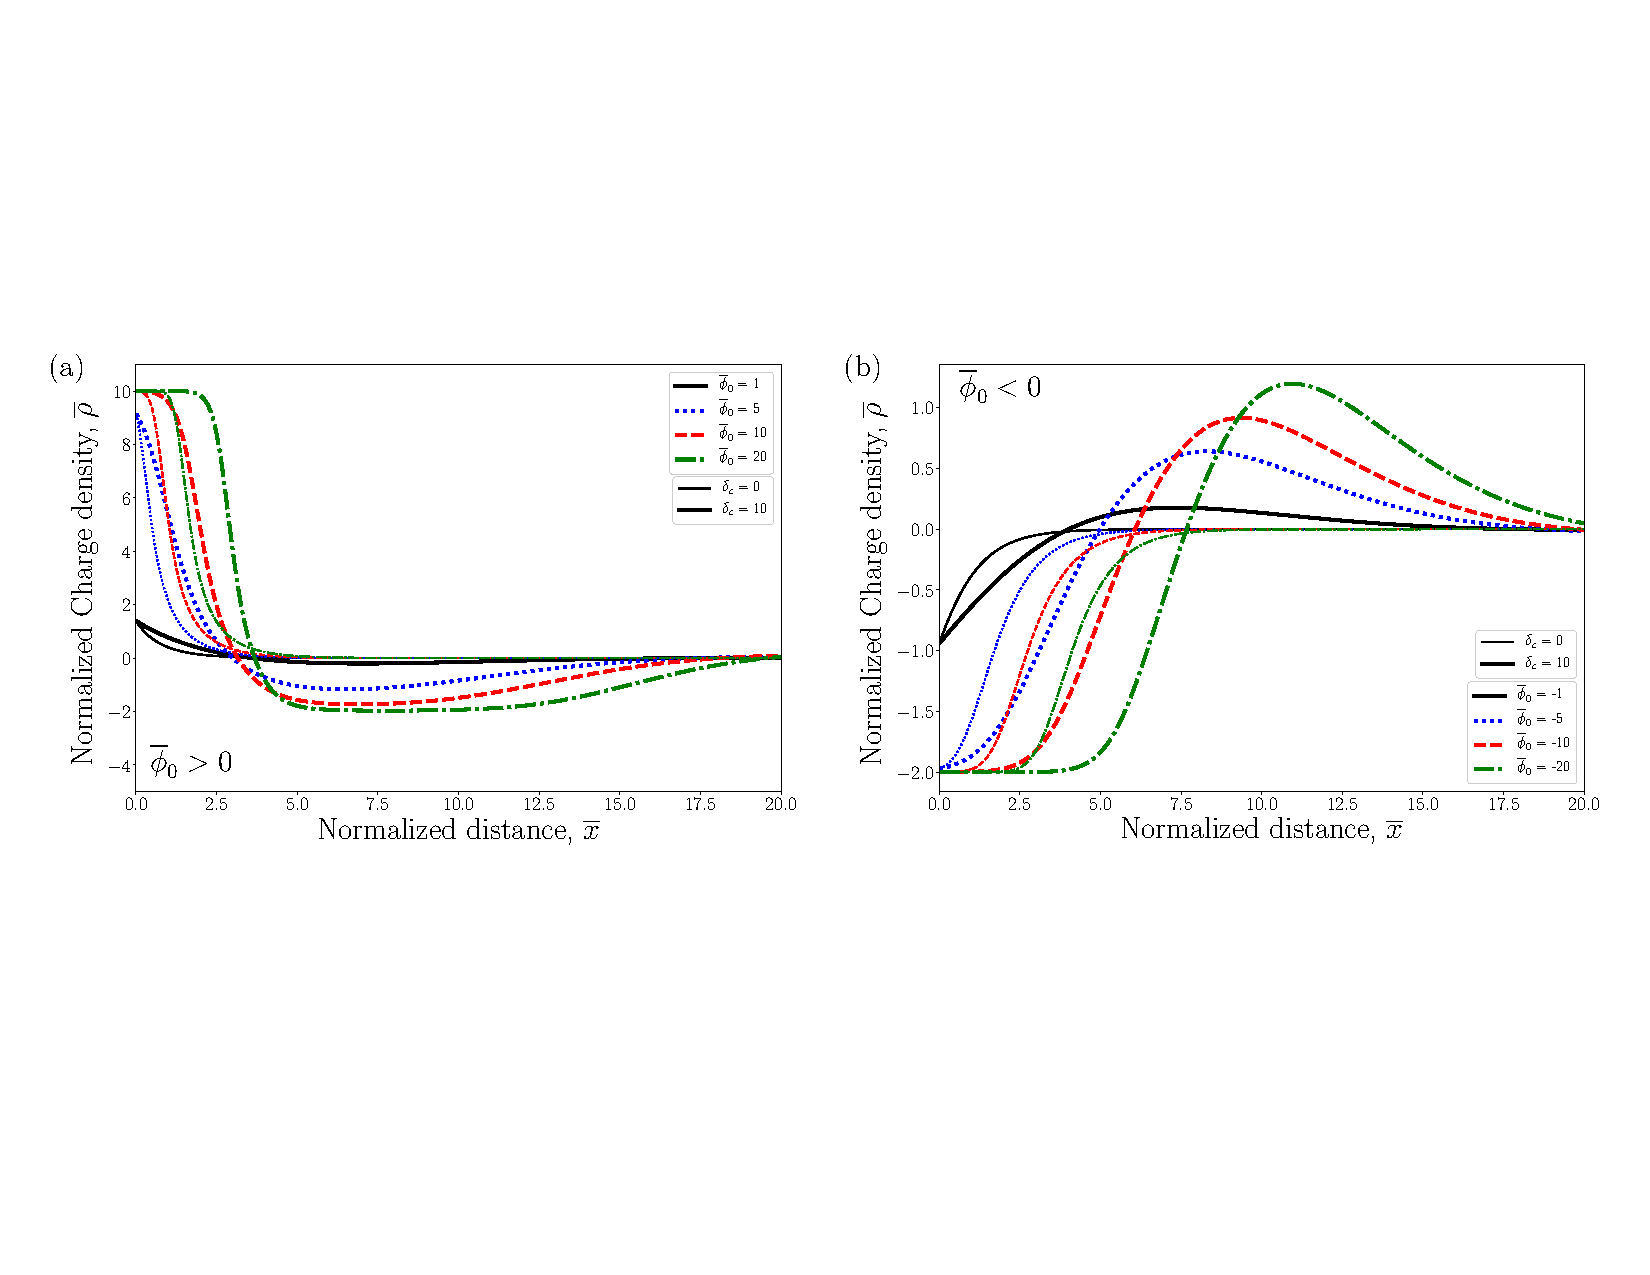
\includegraphics[scale=0.35]{Figure_7.pdf}
         %\caption{ Panel (a): The normalized charge density $\overline{\rho}$ versus the normalized distance $\overline{x}$, Panel (b): same as (a), but with negative initial normalized potential values.}
        %\label{Fig7}
        \end{center}
\end{figure}
\begin{itemize}
    \item $\gamma_+ = 0.5$ and $\gamma_- = 0.1$
    \item Ion crowding effects $\overline{\rho} = \frac{1}{\gamma_\pm}$ and saturation for large $\overline{\phi}_0$
    \item interplay of screening and overcrowding effects for large $\overline{\phi}_0$
\end{itemize}{}
\end{frame}{}

\begin{frame}{Asymmetric Ionic Liquid: Capacitances}
\begin{figure}[!h]
\begin{center}
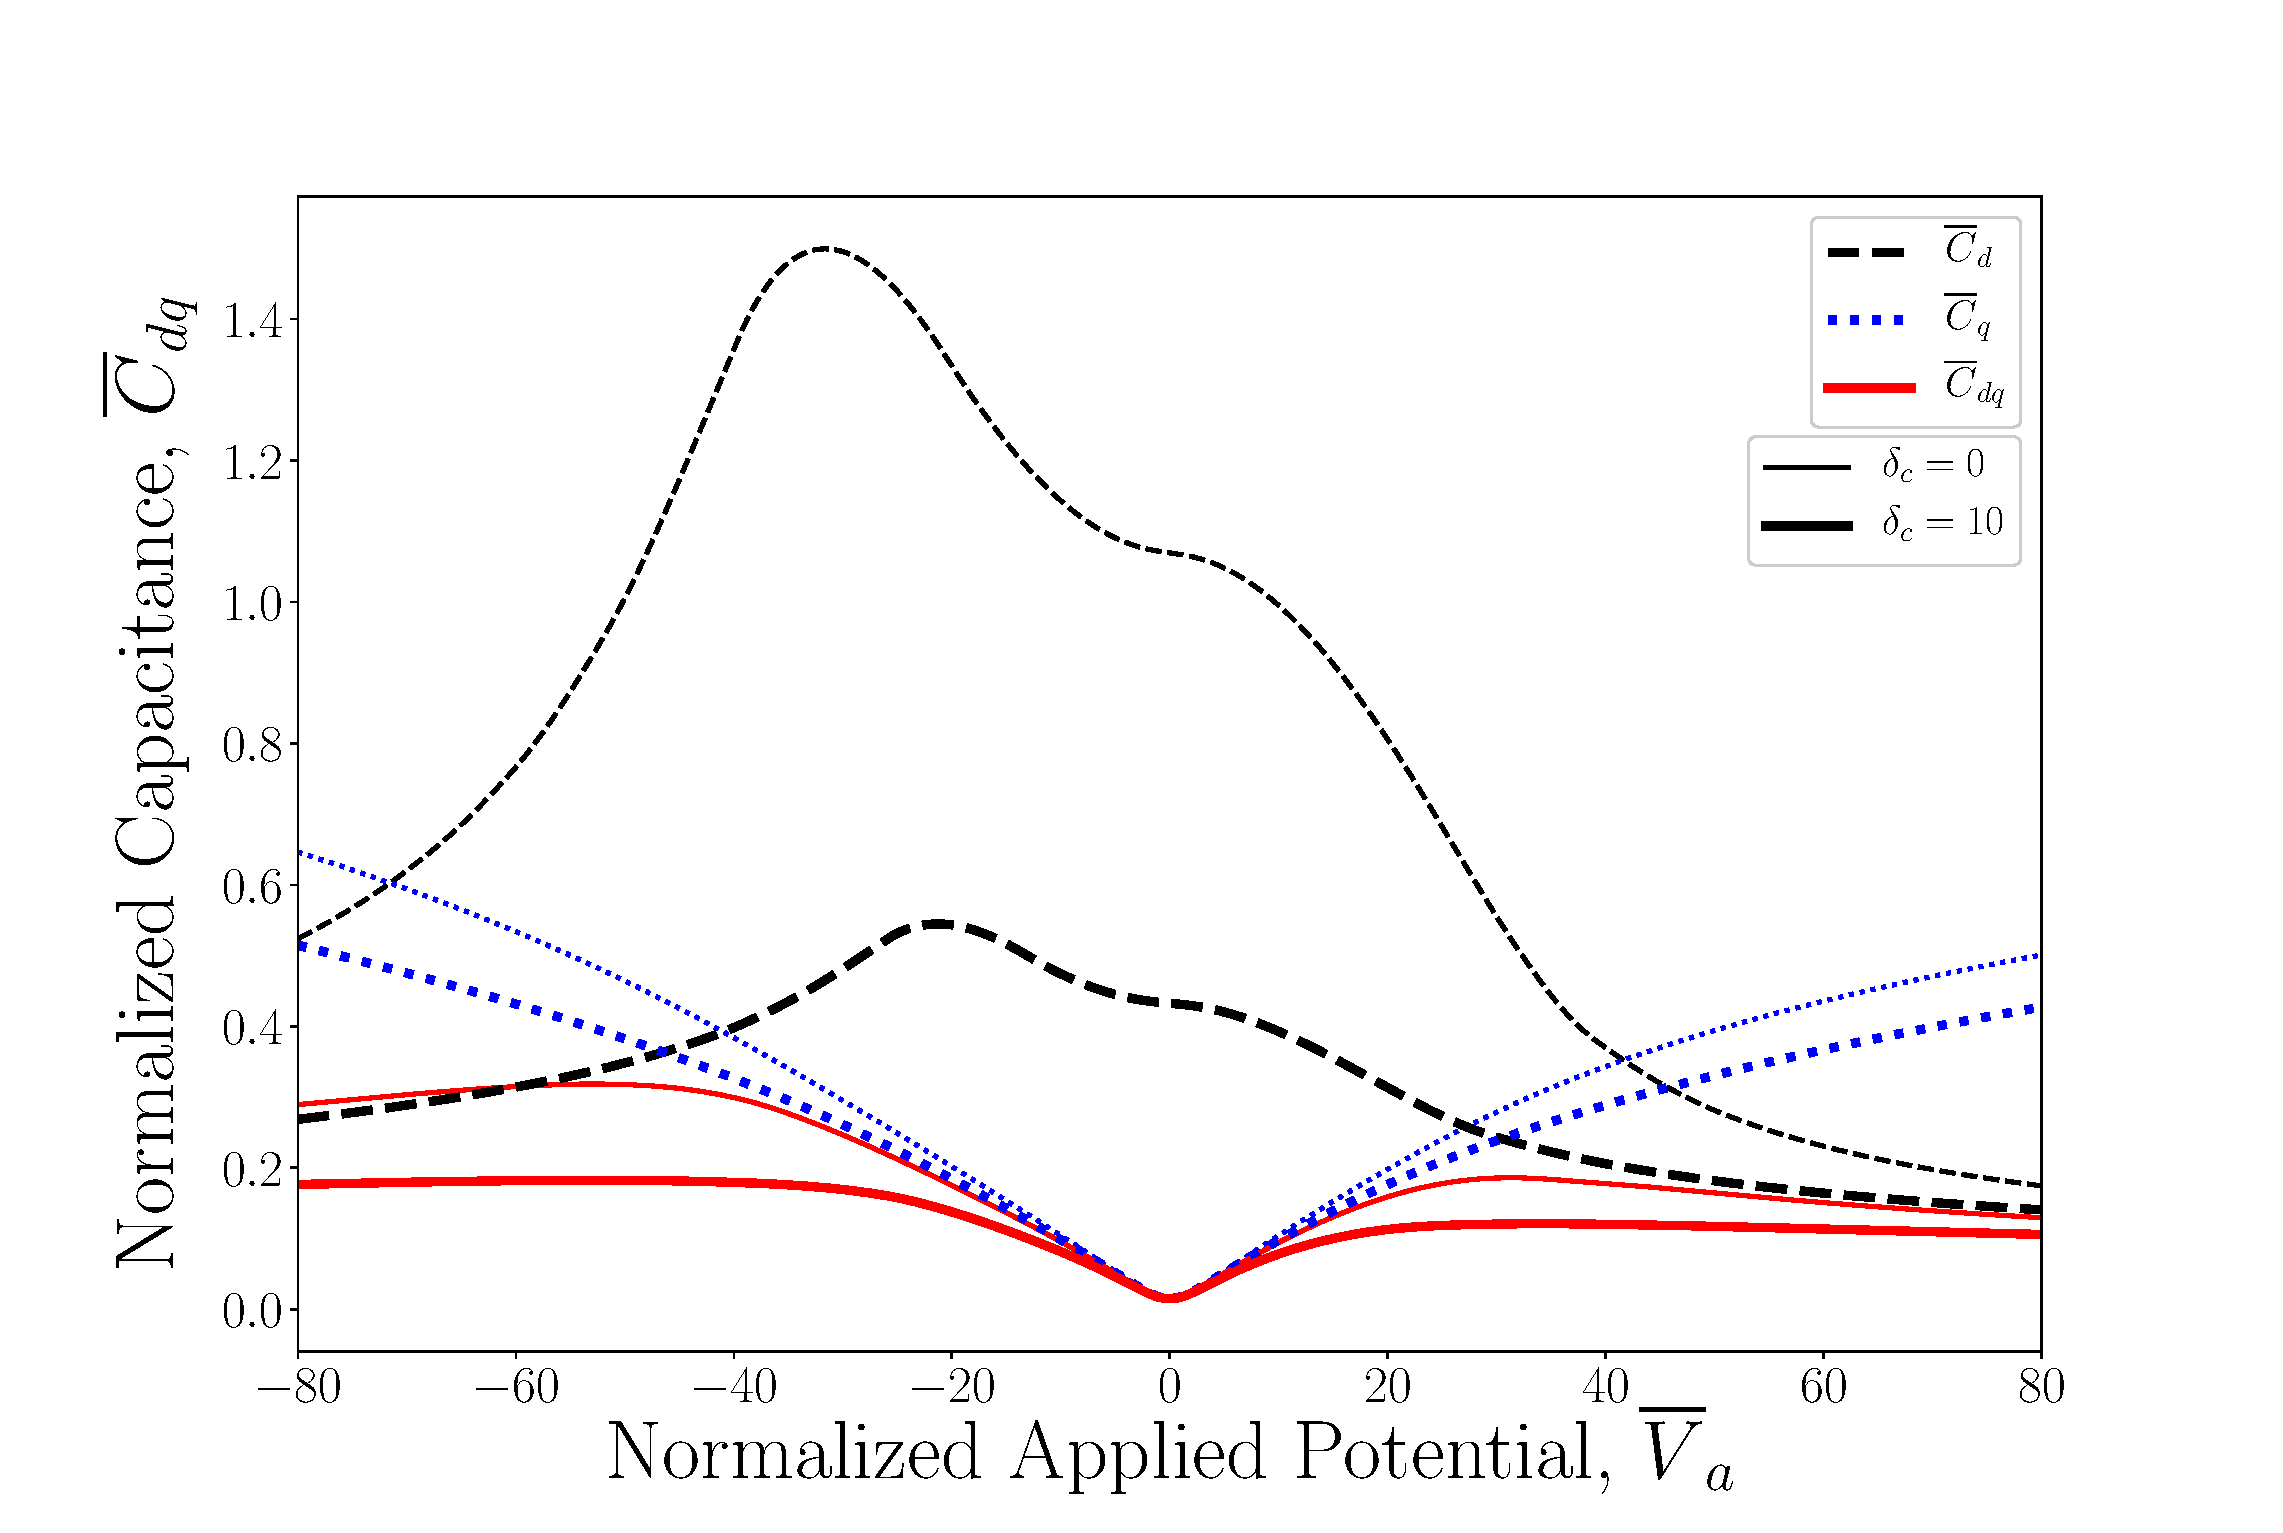
\includegraphics[scale=0.15]{figure_9.eps}
%\caption{ The normalized diffuse capacitance $\overline{C}_d$, quantum capacitance $\overline{C}_q$ and the total capacitance, $\overline{C}_{dq}$ versus the normalized applied potential, $\overline{V}_a $.}
%\label{Fig9}
\end{center}
\end{figure}
\begin{itemize}
    \item Asymmetry in $\overline{C}_d$
    \item $\overline{C}_q$ dominating around the PZC, V-shaped capacitance
    \item For $|\overline{V}_a| > 10$, asymmetric camel shaped $\overline{C}_{dq}$ 
\end{itemize}
\end{frame}{}
%%%%%%%%%%%%%%%% Conclusions %%%%%%%%%%%%%%%%%

\begin{frame}{Outline}

\begin{itemize}
\item Background and Motivation\\
\item Ionic Liquids\\
\item Graphene Electrodes\\
\item Computational approach \\
\item Results \\
\item \textcolor{red}{Conclusions and Future Work}
\end{itemize}
\end{frame}

\section{Conclusions and Future Work}
\begin{frame}{Concluding Remarks}
\begin{itemize}
    \item Ion packing fractions $\gamma = 0.1$ and $\gamma = 0.5$ give rise to camel and bell-shaped diffuse capacitances $C_d$ respectively
    \item Inclusion of Stern layer reduces and broadens the peaks in capacitances
    \item Quantum capacitance $C_g$ dominates around the PZC giving rise to camel shaped capacitances
    \item Asymmetric ionic liquids have asymmetric camel shaped capacitances as well due to $C_g$
\end{itemize}{}
\end{frame}{}

\begin{frame}{Future Work}
\begin{itemize}
    \item Fully asymmetric ionic liquid electrolytes
    \begin{itemize}
        \item Different valency
        \item Different Correlation Lengths
    \end{itemize}{}
    \item Explore New Boundary Conditions
\end{itemize}{}
\end{frame}{}

\begin{frame}{}
    \begin{center}
    Thank you for your attention
    \end{center}
\end{frame}{}

\begin{frame}{Asymmetric Ionic Liquids}
    Consider the case for an asymmetric ionic liquid with equal valency $z_- = z_+ = z$ but unequal ionic volumes $v_-,v_+$
    
    %Unequal ionic volumes only change the entropic term in the free energy functional yielding the following expressions for the concentration:
    $$c_+ = c_{\infty}\frac{e^{-ze\beta \phi}}{g(\phi)}$$
    $$c_- = c_{\infty}\frac{e^{-ze\beta \phi} f(\phi)}{g(\phi)}$$
    where $f(\phi)$ and $g(\phi)$ are given by:
    $$f(\phi) = (1 + \frac{zv_-c_{\infty}}{1 -zv_-c_{\infty}(e^{ze\beta\phi}-1)})^{\frac{v_+}{v_-} -1 } $$
    $$g(\phi) = f(\phi) + zv_+c_{\infty}[e^{-ze\beta\phi}-f(\phi)] +zv_-c_{\infty}f(\phi)(e^{ez\beta\phi} -1)   $$
\end{frame}

\end{document}